% To be compiled with pdflatex.
% This file is to be included into master file via \input command.
% Note that there is no \begin{document} \end{document} brackets!

\newpage
\section{Propagation through atmosphere}
\label{app:Propagation}

\mbox{}

The goal of this section is to develop mathematical models
that can deliver realistic intensity distributions on the Shack-Hartmann WFS
taking into account:
\begin{enumerate}
  \item the intensity distribution in the extended LGS light source formed by
  a specific laser launch telescope and distorted by the upward propagation
  through the turbulent atmosphere;
  \item the phase distortion effects due to atmosphere on the downward light
  path from the LGS to the telescope;
  \item the diffraction effects caused by the main and launch telescope
  apertures, WFS lenslets and the atmospheric turbulence;
  \item anisoplanatic effects due to LGS extent;
  \item scintillation effects due to the atmospheric turbulence.
\end{enumerate}

\subsection{Propagation geometry}

The \texttt{Na} laser guide star is modeled as a set of point sources
distributed within the \texttt{Na} layer and creating the extended light
source shaped as a narrow column inclined with respect to the telescope line
of sight and thus creating elongated images in the focal plane of the
Shack-Hartmann WFS. The details of the LGS geometry are given in Section
\ref{sec:lgs}. Here we note that the point sources that make a LGS are
incoherent and thus the intensity distribution on the detector is a sum of
intensity distributions from each point source. This reduces the problem of
elongated source propagation into a set of point source propagations, so in
what follows we concentrate solely on the problem of the spherical wave
propagation from a point source located at finite distance and shifted with
respect to the telescope optical axis. Another assumption is a layered model
for the atmospheric turbulence. Figure \ref{fig:propagation-geometry} shows
the geometrical configuration used for the modeling. Note that we choose the
turbulence layers orientation to be perpendicular to the telescope optical
axis (see Sec. \ref{subsubsec:perp-turb}).

\begin{figure}[htp]
\begin{center}
 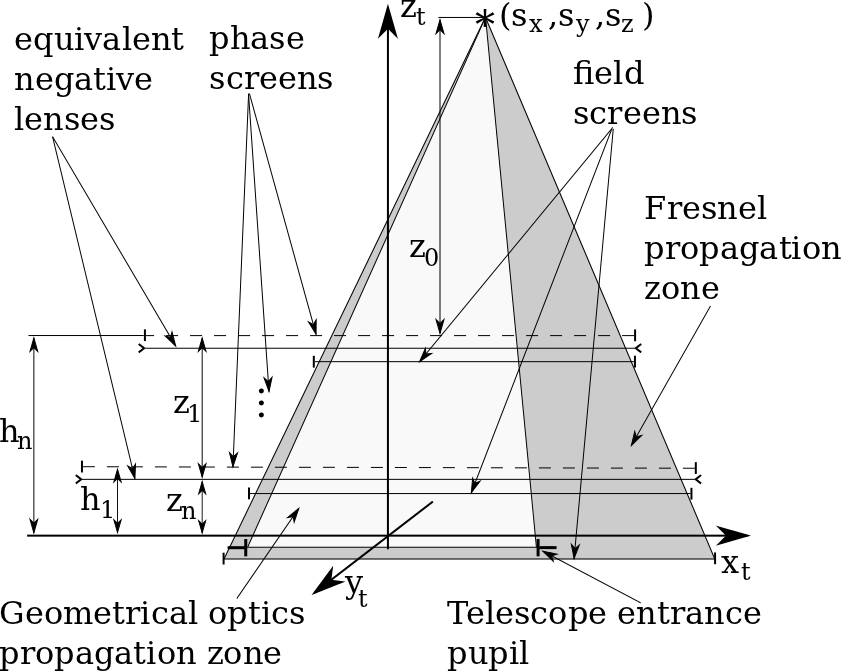
\includegraphics[width = 0.6\textwidth]{Propagation.png}
\end{center}
\caption{Geometry of point source propagation through atmosphere to the
telescope entrance pupil. The orientation corresponds to the \emph{t}-system,
i.e. the \emph{z}-axis is along the telescope optical axis.}
\label{fig:propagation-geometry}
\end{figure}

Light from a point source with coordinates $\bm{s} = (s_{x},s_{y},s_{z})$, and
generally not on the telescope optical axis, propagates through random
atmospheric turbulence phase screens located at altitudes $\{ h_{i}
\}_{i=1}^{n}$ that divide the whole path from the source to the telescope
entrance pupil into a set of propagation paths $\{ z_{j} \}_{j=0}^{n}$.

\subsection{Geometrical optics propagation}

Geometrical optics is a simple approximation that allows e.g. to derive the
relationships between the statistics of the turbulence layers and the optical
field on the sensors.
The geometrical optics propagation is based on the following assumptions:
\begin{itemize}
  \item Light is propagating along straight lines emerging from the point
  source and intersecting the telescope entrance pupil.
  \item Phase distortion along each ray is a sum of phase contributions from each
  phase screen at the point of intersection of the ray and the screen. From
  Figure \ref{fig:propagation-geometry} it is obvious that the coordinates
  $(x,y)$ of the intersection point of ray and phase screen are
  \begin{equation} \label{eq:ray-screen-intersection}
    (x,y) = \frac{(s_{z}-h)}{s_{z}} ( (x_{0},y_{0})-(s_{x},s_{y})
    )+(s_{x},s_{y}),
  \end{equation}
  where $(x_{0},y_{0})$ are the coordinates of a point at the telescope
  entrance pupil, $h$ is the phase screen altitude. Correspondingly, the phase
  deviation from the spherical wavefront at entrance pupil point
  $(x_{0},y_{0})$ is
  \begin{equation} \label{eq:eq:geometrical-phase-deviation}
    \phi (x_{0},y_{0}) = \sum_{i=1}^{n} \phi (x,y)_{i}.
  \end{equation}
  \item Turbulence-induced intensity variations (scintillation) are neglected.
  \item Diffraction effects such as light scattering are not retrievable as
  the geometrical optics propagation is effectively just a scaled projection of
  the phase screens onto the entrance pupil.
\end{itemize}
Normally the phase screens are defined as maps of random phase values on a
point grid. Thus, in order to find the phase at point $(x,y)_{i}$ some or
other interpolation technique is needed. On a regular square grid the bilinear
interpolation is the natural choice.

The geometrical optics propagation zone, i.e. the volume filled with rays that
pass through the telescope entrance pupil, is shown on Figure
\ref{fig:propagation-geometry} in light gray hatch. The minimal physical extent
of a random phase map on each phase screen is defined by the point of
intersection of the propagation zone with the phase screen such that this
point is farthest from the telescope optical axis. Simple geometrical
considerations lead to the estimate for the phase screen diameter
\begin{equation} \label{eq:geometrical-screen-size}
  D_{ps} \geq \frac{(s_{z}-h)}{s_{z}}
  ( D - 2 (s_{x}^{2}+s_{y}^{2})^{1/2}_{max} ) +
  2(s_{x}^{2}+s_{y}^{2})^{1/2}_{max},
\end{equation}
where $D$ is the telescope entrance pupil diameter and maximum is taken over
all the point sources that make the LGS.

\subsection{Generalized Fresnel propagation}

The scalar diffraction using the Fresnel approximation is a more accurate
propagation approach. Fresnel diffraction takes allows to estimate the
scintillation and light scattering effects.

A complication of the diffraction propagation in case of the LGS is the
necessity to effectively address divergence of the wavefronts. A brute force
application of the classical Fresnel integral to the diverging spherical wave
results in excessive sampling requirements. As an optimistic example, consider
the optical
field at the telescope entrance pupil from a pure spherical wave emitted by an
on-axis point source located at altitude of 90 km. In parabolic approximation
the optical field is
$$
  U(\bm{x}) = \exp (i \frac{k}{2z} |\bm{x}|^{2}),
$$
where $k = 2 \pi / \lambda$. The maximal local frequency defining the sampling
is
$$
  f_{max} = \frac{1}{2 \pi} \partial_{x} \left( \frac{k}{2z} |\bm{x}|^{2}
  \right)_{max}
$$
is equal to $\frac{1}{3} \cdot 10^{3}$ m$^{-1}$
for $\lambda = 0.5$ $\mu$m and telescope pupil diameter of 30 m. That is, the
maximal sampling interval in the optical field maps is $\frac{1}{2 f_{max}} =
1.5$ mm, much smaller that the interval needed to adequately sample the
turbulence ($\geq$ 1 cm). This results in unacceptably large $\sim 20K \times
20K$ optical field maps just to sample the oscillations in the spherical wave
amplitude. To avoid this sampling issue the $\exp (i \frac{k}{2z}
|\bm{x}|^{2})$ factor needs to be somehow moved out of the diffraction
integral. This can be done in the
framework of the generalized Fresnel diffraction approach described in
Appendix \ref{app:Fresnel}. Namely, a spherical wave propagation through a
phase screen can be considered a plane wave propagation through a phase screen
and a negative lens with focal distance equal to the curvature radius of the
spherical wavefront at the screen. The propagation through the lens is
governed by the Generalized Fresnel Transform (\ref{eq:GFT-definition}) with
the ABCD-matrix corresponding to the propagation through negative thin lens
with focal distance $f_{1}$ followed by free propagation path of length $z_{1}$:
\begin{equation} \label{eq:lens-free-propagator}
  W = \left[  \begin{array}{cc} 1 & z_{1} \\ 1/f_{1} & 1 \end{array} \right].
\end{equation}
Substituting $W$ from Eq. (\ref{eq:lens-free-propagator}) into the
Cast-to-Convolution theorem or, equivalently, using first Focus and then
Cast-to-convolution theorem, we find that after propagation through the phase
screen-lens combination the diffracted field has the necessary factorized form
\begin{equation} \label{eq:factorized-field}
  U(\bm{x}) = \exp (i\frac{k}{2 f_{2}} |\bm{x}|^{2}) \tilde{U} (\bm{x}),
\end{equation}
where $f_{2} = f_{1}+z_{1}$, $\tilde{U} (\bm{x})$ is a plane wave field 1)
multiplied by the first phase screen, 2) Fresnel-propagated distance $z_{1}
\frac{f_{1}}{z_{1}+f_{1}}$ to the next screen and 3) scaled by
factor $\frac{f_{1}+z_{1}}{f_{{1}}}$ (see Eq.
\ref{eq:convolution-cast}). Obviously, the next propagation step is
identical to the first one after replacing $z_{1}$ with $z_{2}$ and $f_{1}$
with $f_{2}$, etc. Since the $\tilde{U}$-field is diffraction
of the plane wave (multiplied by the turbulence random phase mask), the
sampling requirements are significantly relaxed. Note that $f_{i}$ in the
parabolic phase
factor $\exp (i\frac{k}{2f_{i}} |\bm{x}|^{2})$ on each screen is equal just to
the distance
to the point source, i.e. represents the un-diffracted spherical wave complex
amplitude on each
screen; the scaling factor $\frac{f_{i}+z_{i}}{f_{i}}$ just shows how much the
grid on $i$th screen expands when projected on $(i+1)$th screen along the rays
emerging from the spherical wave center.

These observations allow to define a recursive algorithm for the diverging
spherical wave diffraction by a sequence of turbulence phase screens. For more
generality we assume that the propagation from turbulent phase screen $i$ to
screen $i+1$ is not necessarily free-space but is governed by a non-trivial
wave matrix $W_{i}$. We also need to take into account that propagation from
multiple point sources making the LGS extended light source is done through
the same turbulence volume, i.e. through the same set of phase screens. To
take into account the shift of each point source with respect to the telescope
optical axis it is best to perform propagation from this source in the shifted
coordinate system in which the source is at $(0,0,h_{s})$ and to use
interpolation to first read the phase values from the phase screen to the
shifted field map and, in the end, to read the values from the propagated
field map onto the entrance pupil grid. The following data/operation flow is
assumed:
\begin{enumerate}
  \item Preparational stage.
  \begin{itemize}
    \item Define a set of the point sources making up a LGS: their
    $\{ (s_{x},s_{y},s_{z})_{s} \}_{s=1}^{\#PtS}$-coordinates and relative
    intensities (weights) $\{ w_{s} \}_{s=1}^{\#PtS}$.
    \item Set a working wavelength $\lambda$.
    \item Define a turbulence model: number of turbulence layers, their
    altitudes $\{ h_{p} \}_{p=1}^{\#PS}$, partial turbulence strengths via Fried
    parameters of $C_{n}^{2}$, inner and outer scales, etc.
    \item Define a set of layer-to-layer propagation wave matrices $\{ W_{p}
    \}_{p=1}^{\#PS}$. In case of free-space propagation between layers, the
    matrices are
    \begin{equation} \label{eq:free-propagation-matrices}
      W_{p} = \left[ \begin{array}{cc} 1 & z_{p} \\ 0 & 1 \end{array} \right],
    \end{equation}
    where $\{ z_{p} \}_{p=1}^{\#PS}$ are distances between layers, $z_{1}$
    is the distance between last layer and the entrance pupil.
    \item Generate a set $\{ P_{p} \}_{p=1}^{\#PS}$ of the random phase screens
    on each turbulence layer. The key
    parameters for this operation are the physical size of each screen and its
    sampling interval $dx_{p}$. We note that, because of interpolation operation
    assumed to read
    from the phase screen into the optical field, the sampling of the screens
    does not have to be the same or equal to the optical field map sampling and
    can follow the natural sampling conditions on each screen
    \begin{equation} \label{eq:phase-screen-sampling}
      dx_{p} = r_{0_{p}} / m, \,\, p = 1,...,\#PS,
    \end{equation}
    where $r_{0_{p}}$ is a partial Fried parameter for each screen, $m$-factor
    varies from 5 to 10. The physical size of each screen is determined by the
    ``Fresnel propagation'' zone shown on Figure \ref{fig:propagation-geometry}.
    From the picture we see that the safe value for diameter $D_{p}$ of a phase
    screen located at altitude $h_{p}$ should be
    \begin{equation} \label{eq:phase-screen-size}
      D_{p} \geq g D + 3 (s_{x}^{2}+s_{y}^{2})^{1/2}_{max},
    \end{equation}
    where $D$ is the entrance pupil diameter, $g$ is an oversize or ``guard''
    factor ($g > 1$), $h_{0}$ is the point source
    altitude, and the maximum is taken over all the point sources.
  \end{itemize}
  \item Loop over point sources.
  \begin{itemize}
    \item Find the focal distance of the equivalent negative lens on the first
    phase screen to propagate (which is the highest one!):
    \begin{equation} \label{eq:initial-f}
      f_{\#PS} = s_{z}-h_{\#PS},
    \end{equation}
    where $s_{z}$ is the $z$-coordinate (altitude) of the current point source.
    \item Run the ``propagation parameter recursion'':
    \begin{equation} \label{eq:W-recursion}
      \tilde{W}_{p} = W_{p} +
      \left[
      \begin{array}{cc} B_{p}/f_{p} & 0 \\ D_{p}/f_{p} & 0 \end{array}
      \right],
    \end{equation}
    $$ f_{p-1} = \frac{\tilde{A}_{p}}{\tilde{C}_{p}}, \,\, p = \#PS,...,1, $$
    where $W_{p}$ are the ABCD-matrices defined at the preparatory stage,
    $\tilde{W}_{p}$ are the ``spherical wave propagation'' ABCD-matrices
    formed according to Eqs. (\ref{eq:focus-theorem},
    \ref{eq:convolution-cast}). Note the descending layer counter. The
    $\{ (\tilde{W}_{p},f_{p}) \}_{p=1}^{\#PS}$-set
    completely defines parameters for spherical wave propagation through all
    the phase screens to the telescope entrance pupil by Eq.
    (\ref{eq:convolution-cast}), $f_{0}$ defines the curvature of the
    spherical wave factor (see Eq. (\ref{eq:factorized-field})) in the
    entrance pupil, the $\tilde{B}_{p}/\tilde{A}_{p}$ is the equivalent
    propagation distance from layer $p$ to layer $p+1$, $\tilde{A}_{p}$ is the
    field grid expansion factor from layer $p$ to $p+1$.
    \item Decide on the size and sampling interval for the field amplitude map
    to propagate. Generally, these parameters depend on the point source so
    this stage resides in the point source loop. We make the following
    observations:
    \begin{itemize}
      \item In order to use FFT to evaluate the convolution in Eq.
      (\ref{eq:convolution-cast}) the \emph{pixel} size $N$ of field map on
      each screen should be the same (otherwise an additional interpolation is
      needed). The physical size, however, is different on each screen, it is
      scaled by factor $\tilde{A}_{p}$. In the entrance pupil the physical
      field map size is
      \begin{equation} \label{eq:field-map-scaling}
        \tilde{D}_{0} = \tilde{D}_{\#PS} \prod_{p=1}^{\#PS} \tilde{A}_{p},
      \end{equation}
      where $\tilde{D}_{\#PS}$ is the diameter of the field map on the highest
      phase screen from where the propagation starts. According to Figure
      \ref{fig:propagation-geometry}
      \begin{equation} \label{eq:field-map-size}
        \tilde{D}_{0} \geq g D + (s_{x}^{2}+s_{y}^{2})^{1/2}_{max}.
      \end{equation}
      \item Likewise, if the spacing on the highest field screen is decided to
      be equal to $dx_{\#PS}$, then the spacing on the same field screen
      propagated down to the entrance pupil will be
      \begin{equation} \label{eq:field-map-spacing}
        dx_{0} = dx_{\#PS} \prod_{p=1}^{\#PS} \tilde{A}_{p}.
      \end{equation}
      Since $\tilde{A}_{p} \geq 1$, $\forall i$, for the most typical case of
      free-space propagation of
      the diverging spherical wave, $dx_{0} \geq dx_{\#PS}$ but
      it is the last field screen that needs to be sampled the finest to
      represent the field distorted by the whole volume of the turbulence. So
      it would be wise to first
      choose $dx_{0}$ as a fraction of the Fried parameter $r_{0}$ for
      the whole turbulence volume then find $dx_{\#PS}$ on the first screen to
      propagate from Eq. (\ref{eq:field-map-spacing}).
    \end{itemize}
    Thus, using Eq. (\ref{eq:field-map-size}) we decide on the field map
    physical size, choose $dx_{0}$, find the field map pixel size as
    \begin{equation} \label{eq:field-map-pixels}
      N = ceiling( \tilde{D}_{0}/dx_{0} )
    \end{equation}
    and find $dx_{\#PS}$ from Eq. (\ref{eq:field-map-spacing}) for the
    beginning of propagation sequence.
    \item Generate the Generalized Fresnel propagator maps $\{ H_{p}
    \}_{p=1}^{\#PS}$. Note that this
    stage is sitting inside the point source loop because map spacings depend
    on the position of the current point source!
    \begin{equation} \label{eq:propagator-sequence}
      df_{p} = \frac{1}{N dx_{p}},
    \end{equation}
    $$ \alpha_{p} = \frac{\tilde{A}_{p}}{\lambda \tilde{B}_{p}}, $$
    $$ H_{p,mn} = \frac{i}{\alpha} \exp \left( -i \frac{\pi}{\alpha}
    ((mdf_{p})^{2}+(mdf_{p})^{2}) \right), \,\, i = \sqrt{-1}, $$
    $$ dx_{p-1} = \tilde{A}_{p} dx_{p}, $$
    $$ p = \#PS,...,1, \,\, m,n = -N/2,...,N/2. $$
    Factor $i/\alpha$ can be omitted. Note the descending layer counter.
    \item Perform actual propagation of $\tilde{U}$-field (see Eq.
    \ref{eq:factorized-field}) down to the entrance pupil:
    \begin{equation} \label{eq:fresnel-propagation}
      x_{mn} = ( n dx_{p} + s_{x} )/dp_{p},
    \end{equation}
    $$ y_{mn} = ( m dx_{p} + s_{y} )/dp_{p}, $$
    $$ \tilde{U}_{mn} \leftarrow \tilde{U}_{mn}
      \exp \left[ i \mathbb{B}(P_{p},x_{mn},y_{mn}) \right], $$
    $$ \tilde{U} \leftarrow \mathbb{F} \left( \tilde{U} \right), $$
    $$ \tilde{U} \leftarrow \tilde{U} H_{p}, $$
    $$ \tilde{U} \leftarrow \mathbb{F}^{-1} \left( \tilde{U} \right), $$
    $$ p = \#PS,...,1, \,\, m,n = -N/2,...,N/2, $$
    where $\leftarrow$ means ``in-place'' operation, $\mathbb{B}$ is the
    standard bilinear interpolation operator assuming that the map to
    interpolate \emph{from} has unit spacing (other sort of interpolation can
    be used, of course), $dp_{p}$ is the $p$th phase screen spacing,
    $\mathbb{F}$ is the Fourier transform operator.
    \item Interpolate the $\tilde{U}$-field defined on the shifted grid in the
    entrance pupil onto the another grid in the entrance pupil convenient for
    subsequent propagation through Shack-Hartmann WFS lenslets:
    \begin{equation} \label{eq:pupil-interpolation}
      x_{mn} = ( m dx - s_{x} + l_{x} )/dx_{0},
    \end{equation}
    $$ y_{mn} = ( n dx - s_{y} + l_{y} )/dx_{0}, $$
    $$ \tilde{G}_{mn} = \mathbb{B}(\tilde{U},x_{mn},y_{mn}), $$
    $$ m,n = -M/2,...,M/2, $$
    where $dx$ and $M$ are the spacing and pixel size of the ``lenslet map''
    grid, $(l_{x},l_{y})$ is the lenslet map grid shift with respect to the
    pupil center. Then
    \begin{equation} \label{eq:full-entrance-field}
      G_{mn} = \exp \left[ -i \frac{k}{2f_{0}} (x_{mn}^{2}+y_{mn}^{2}) \right]
      \tilde{G}_{mn},
    \end{equation}
    $$ x_{mn} = ndx - s_{x} + l_{x}, \,\, y_{mn} = mdx - s_{y} + l_{y},
       \,\, m,n = -M/2,M/2. $$
  \end{itemize}
  is the full field in the entrance pupil propagated from the current point
  source. This is the end of the propagation calculation for a single point
  source. Note that the last stage (the interpolation to lenslet map) can be
  omitted and attached to the next stage, the propagation through WFS
  lenslets. In this case the $\tilde{U}$-field is the final output of Fresnel
  propagation to the entrance pupil, which together with source
  \emph{xy}-shift $(s_{x},s_{y})$, pupil grid spacing $dx_{0}$ and the
  spherical wavefront equivalent focal distance $f_{0}$ are the outputs of this
  algorithm.
\end{enumerate}